% Options for packages loaded elsewhere
\PassOptionsToPackage{unicode}{hyperref}
\PassOptionsToPackage{hyphens}{url}
\PassOptionsToPackage{dvipsnames,svgnames,x11names}{xcolor}
%
\documentclass[
  11pt,
]{article}

\usepackage{amsmath,amssymb}
\usepackage{iftex}
\ifPDFTeX
  \usepackage[T1]{fontenc}
  \usepackage[utf8]{inputenc}
  \usepackage{textcomp} % provide euro and other symbols
\else % if luatex or xetex
  \usepackage{unicode-math}
  \defaultfontfeatures{Scale=MatchLowercase}
  \defaultfontfeatures[\rmfamily]{Ligatures=TeX,Scale=1}
\fi
\usepackage{lmodern}
\ifPDFTeX\else  
    % xetex/luatex font selection
\fi
% Use upquote if available, for straight quotes in verbatim environments
\IfFileExists{upquote.sty}{\usepackage{upquote}}{}
\IfFileExists{microtype.sty}{% use microtype if available
  \usepackage[]{microtype}
  \UseMicrotypeSet[protrusion]{basicmath} % disable protrusion for tt fonts
}{}
\makeatletter
\@ifundefined{KOMAClassName}{% if non-KOMA class
  \IfFileExists{parskip.sty}{%
    \usepackage{parskip}
  }{% else
    \setlength{\parindent}{0pt}
    \setlength{\parskip}{6pt plus 2pt minus 1pt}}
}{% if KOMA class
  \KOMAoptions{parskip=half}}
\makeatother
\usepackage{xcolor}
\usepackage[margin=1in]{geometry}
\setlength{\emergencystretch}{3em} % prevent overfull lines
\setcounter{secnumdepth}{-\maxdimen} % remove section numbering
% Make \paragraph and \subparagraph free-standing
\ifx\paragraph\undefined\else
  \let\oldparagraph\paragraph
  \renewcommand{\paragraph}[1]{\oldparagraph{#1}\mbox{}}
\fi
\ifx\subparagraph\undefined\else
  \let\oldsubparagraph\subparagraph
  \renewcommand{\subparagraph}[1]{\oldsubparagraph{#1}\mbox{}}
\fi


\providecommand{\tightlist}{%
  \setlength{\itemsep}{0pt}\setlength{\parskip}{0pt}}\usepackage{longtable,booktabs,array}
\usepackage{calc} % for calculating minipage widths
% Correct order of tables after \paragraph or \subparagraph
\usepackage{etoolbox}
\makeatletter
\patchcmd\longtable{\par}{\if@noskipsec\mbox{}\fi\par}{}{}
\makeatother
% Allow footnotes in longtable head/foot
\IfFileExists{footnotehyper.sty}{\usepackage{footnotehyper}}{\usepackage{footnote}}
\makesavenoteenv{longtable}
\usepackage{graphicx}
\makeatletter
\def\maxwidth{\ifdim\Gin@nat@width>\linewidth\linewidth\else\Gin@nat@width\fi}
\def\maxheight{\ifdim\Gin@nat@height>\textheight\textheight\else\Gin@nat@height\fi}
\makeatother
% Scale images if necessary, so that they will not overflow the page
% margins by default, and it is still possible to overwrite the defaults
% using explicit options in \includegraphics[width, height, ...]{}
\setkeys{Gin}{width=\maxwidth,height=\maxheight,keepaspectratio}
% Set default figure placement to htbp
\makeatletter
\def\fps@figure{htbp}
\makeatother
\newlength{\cslhangindent}
\setlength{\cslhangindent}{1.5em}
\newlength{\csllabelwidth}
\setlength{\csllabelwidth}{3em}
\newlength{\cslentryspacingunit} % times entry-spacing
\setlength{\cslentryspacingunit}{\parskip}
\newenvironment{CSLReferences}[2] % #1 hanging-ident, #2 entry spacing
 {% don't indent paragraphs
  \setlength{\parindent}{0pt}
  % turn on hanging indent if param 1 is 1
  \ifodd #1
  \let\oldpar\par
  \def\par{\hangindent=\cslhangindent\oldpar}
  \fi
  % set entry spacing
  \setlength{\parskip}{#2\cslentryspacingunit}
 }%
 {}
\usepackage{calc}
\newcommand{\CSLBlock}[1]{#1\hfill\break}
\newcommand{\CSLLeftMargin}[1]{\parbox[t]{\csllabelwidth}{#1}}
\newcommand{\CSLRightInline}[1]{\parbox[t]{\linewidth - \csllabelwidth}{#1}\break}
\newcommand{\CSLIndent}[1]{\hspace{\cslhangindent}#1}

\makeatletter
\makeatother
\makeatletter
\makeatother
\makeatletter
\@ifpackageloaded{caption}{}{\usepackage{caption}}
\AtBeginDocument{%
\ifdefined\contentsname
  \renewcommand*\contentsname{Table of contents}
\else
  \newcommand\contentsname{Table of contents}
\fi
\ifdefined\listfigurename
  \renewcommand*\listfigurename{List of Figures}
\else
  \newcommand\listfigurename{List of Figures}
\fi
\ifdefined\listtablename
  \renewcommand*\listtablename{List of Tables}
\else
  \newcommand\listtablename{List of Tables}
\fi
\ifdefined\figurename
  \renewcommand*\figurename{Figure}
\else
  \newcommand\figurename{Figure}
\fi
\ifdefined\tablename
  \renewcommand*\tablename{Table}
\else
  \newcommand\tablename{Table}
\fi
}
\@ifpackageloaded{float}{}{\usepackage{float}}
\floatstyle{ruled}
\@ifundefined{c@chapter}{\newfloat{codelisting}{h}{lop}}{\newfloat{codelisting}{h}{lop}[chapter]}
\floatname{codelisting}{Listing}
\newcommand*\listoflistings{\listof{codelisting}{List of Listings}}
\makeatother
\makeatletter
\@ifpackageloaded{caption}{}{\usepackage{caption}}
\@ifpackageloaded{subcaption}{}{\usepackage{subcaption}}
\makeatother
\makeatletter
\@ifpackageloaded{tcolorbox}{}{\usepackage[skins,breakable]{tcolorbox}}
\makeatother
\makeatletter
\@ifundefined{shadecolor}{\definecolor{shadecolor}{rgb}{.97, .97, .97}}
\makeatother
\makeatletter
\makeatother
\makeatletter
\makeatother
\ifLuaTeX
  \usepackage{selnolig}  % disable illegal ligatures
\fi
\IfFileExists{bookmark.sty}{\usepackage{bookmark}}{\usepackage{hyperref}}
\IfFileExists{xurl.sty}{\usepackage{xurl}}{} % add URL line breaks if available
\urlstyle{same} % disable monospaced font for URLs
\hypersetup{
  pdftitle={Quarto},
  pdfauthor={Wojciech Hardy},
  colorlinks=true,
  linkcolor={blue},
  filecolor={Maroon},
  citecolor={Blue},
  urlcolor={Blue},
  pdfcreator={LaTeX via pandoc}}

\title{Quarto}
\usepackage{etoolbox}
\makeatletter
\providecommand{\subtitle}[1]{% add subtitle to \maketitle
  \apptocmd{\@title}{\par {\large #1 \par}}{}{}
}
\makeatother
\subtitle{PDF and LaTeX}
\author{Wojciech Hardy}
\date{2023-04-27}

\begin{document}
\maketitle
\ifdefined\Shaded\renewenvironment{Shaded}{\begin{tcolorbox}[sharp corners, frame hidden, enhanced, breakable, boxrule=0pt, borderline west={3pt}{0pt}{shadecolor}, interior hidden]}{\end{tcolorbox}}\fi

\begin{center}\rule{0.5\linewidth}{0.5pt}\end{center}

\hypertarget{pdf}{%
\subsection{PDF}\label{pdf}}

PDFs are created using LaTeX. As such some `dynamic' fields don't work
here. But also, we get to use TeX for formatting.

\hypertarget{pdf-specifc-options}{%
\subsubsection{PDF-specifc options}\label{pdf-specifc-options}}

Changing the font size:

\texttt{fontsize:\ 11pt}

Changing the margins:

\texttt{geometry:\ margin=1in}

(These actually modify LaTeX template options).

\begin{center}\rule{0.5\linewidth}{0.5pt}\end{center}

\hypertarget{latex-related}{%
\subsubsection{LaTeX-related}\label{latex-related}}

We can set the document type.

\texttt{documentclass:\ article}

(alternatives include \texttt{letter}, \texttt{book}, \texttt{slides},
\texttt{beamer}, etc.)

\begin{center}\rule{0.5\linewidth}{0.5pt}\end{center}

We can change the engine used to produce the output, e.g.:

\texttt{pdf:}\strut \\
\texttt{latex\_engine:\ xelatex}

\begin{center}\rule{0.5\linewidth}{0.5pt}\end{center}

We can tell RMarkdown to keep the intermediate \texttt{.tex} file.

\texttt{pdf:}\strut \\
\texttt{keep\_tex:\ true}

(Note: similarly, we can keep the \texttt{.md} file for non-pdf formats
with \texttt{keep\_md:\ true})

\begin{center}\rule{0.5\linewidth}{0.5pt}\end{center}

We can use \texttt{LaTeX} directly within the document and it will be
processed using the chosen engine.

\texttt{\textbackslash{}begin\{center\}\ \%center}\strut \\
\texttt{\textbackslash{}includegraphics{[}width=10cm,\ height=6cm,\ keepaspectratio{]}\{img/chart.png\}}\strut \\
\texttt{(source:\ https://www.tylervigen.com/spurious-correlations)}\strut \\
\texttt{\textbackslash{}end\{center\}}\strut \\
\texttt{\textbackslash{}newpage}\strut \\
\texttt{\textbackslash{}Large\ Large\ letters}\strut \\
\texttt{\textbackslash{}footnote\{This\ is\ a\ footnote\}}

\begin{center} %center
  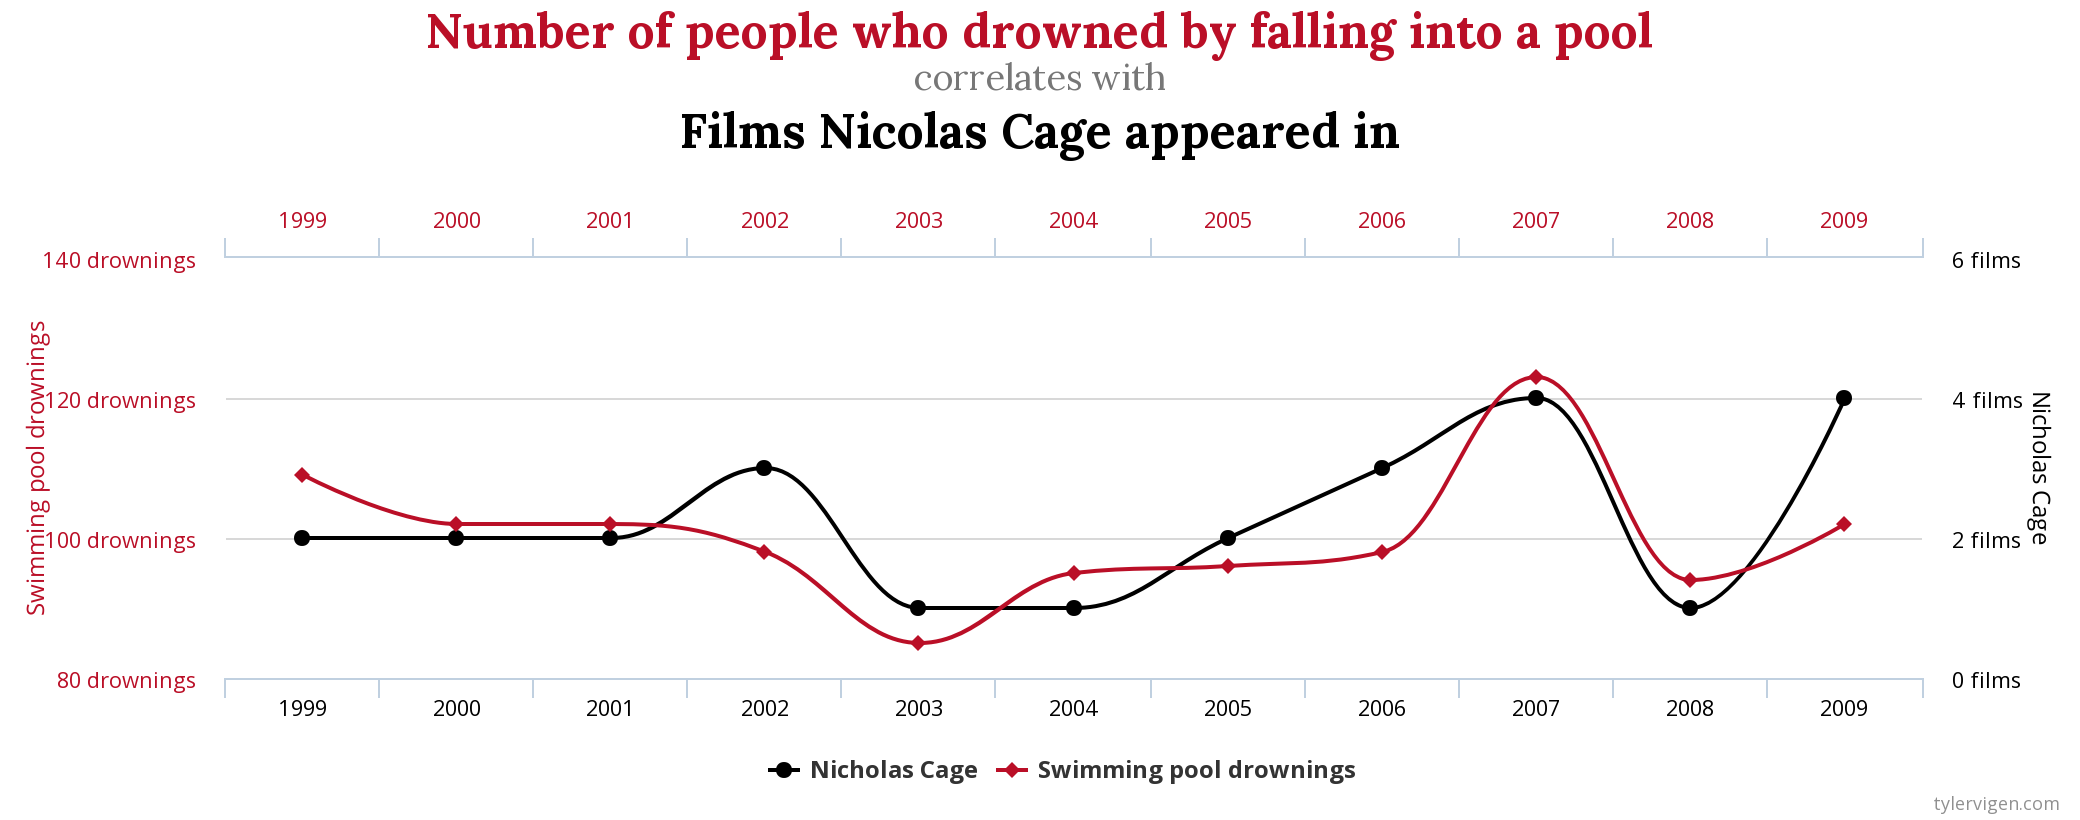
\includegraphics[width=10cm, height=6cm, keepaspectratio]{../img/chart.png}  
(source: https://www.tylervigen.com/spurious-correlations)
\end{center}
\newpage

\Large Large letters \footnote{This is a footnote}

\begin{center}\rule{0.5\linewidth}{0.5pt}\end{center}

You may also use the LaTeX citation syntax. We need to specify what
package do we want to use to manage the citations, e.g.:

\texttt{pdf\_document:}\strut \\
\texttt{citation\_package:\ natbib}

\paragraph{QMD}

\texttt{Studies\ concerning\ other\ cultural\ goods\ exploit\ quasi-natural\ experiments\ of\ policy\ and\ institutional\ changes.\ One\ example\ of\ the\ policy\ change\ is\ the\ introduction\ of\ download\ penalization\ in\ France\ (HADOPI),\ as\ scrutinized\ by\ @danaher\_effect\_2012.\ The\ analyzed\ cases\ of\ institutional\ change\ include\ the\ sudden\ and\ transitory\ disappearance\ of\ the\ NBC\ content\ from\ iTunes\ {[}@danaher\_converting\_2010{]}\ as\ well\ as\ the\ Megaupload\ shutdown\ {[}@danaher\_gone\_2014;\ @peukert\_piracy\_2013{]}\ and\ website\ blocking\ in\ the\ UK\ {[}@danaher\_website\_2016{]}.\ Interestingly,\ @danaher\_gone\_2014\ and\ @peukert\_piracy\_2013\ analyzing\ the\ same\ case\ of\ Megaupload\ shutdown\ come\ to\ rather\ different\ conclusions:\ the\ former\ find\ that\ the\ shutdown\ caused\ an\ increase\ in\ digital\ downloads\ from\ legal\ sources;\ the\ latter\ finds\ no\ change\ in\ box\ office\ revenue.\ This\ difference\ could\ be\ attributed\ to\ the\ fact\ that\ a\ downloaded\ "pirated"\ copy\ may\ be\ a\ perfect\ substitute\ for\ a\ copy\ downloaded\ from\ a\ legitimate\ source,\ but\ not\ for\ a\ visit\ to\ the\ movie\ theater.\ @danaher\_website\_2016\ argue\ that\ only\ large\ scale\ interventions\ (such\ as\ blocking\ multiple\ websites\ with\ unauthorized\ distribution)\ appear\ noticeably\ reduce\ "piracy"\ and\ raise\ paid\ consumption,\ but\ these\ effects\ are\ only\ transitory.}

\paragraph{Output}

Studies concerning other cultural goods exploit quasi-natural
experiments of policy and institutional changes. One example of the
policy change is the introduction of download penalization in France
(HADOPI), as scrutinized by Danaher et al. (2014). The analyzed cases of
institutional change include the sudden and transitory disappearance of
the NBC content from iTunes (Danaher et al. 2010) as well as the
Megaupload shutdown (Danaher and Smith 2014; Peukert, Claussen, and
Kretschmer 2017) and website blocking in the UK (Danaher, Smith, and
Telang 2016). Interestingly, Danaher and Smith (2014) and Peukert,
Claussen, and Kretschmer (2017) analyzing the same case of Megaupload
shutdown come to rather different conclusions: the former find that the
shutdown caused an increase in digital downloads from legal sources; the
latter finds no change in box office revenue. This difference could be
attributed to the fact that a downloaded ``pirated'' copy may be a
perfect substitute for a copy downloaded from a legitimate source, but
not for a visit to the movie theater. Danaher, Smith, and Telang (2016)
argue that only large scale interventions (such as blocking multiple
websites with unauthorized distribution) appear noticeably reduce
``piracy'' and raise paid consumption, but these effects are only
transitory.

\hypertarget{bibliography}{%
\section{Bibliography}\label{bibliography}}

The cited works get pasted here.

\hypertarget{refs}{}
\begin{CSLReferences}{1}{0}
\leavevmode\vadjust pre{\hypertarget{ref-danaher_converting_2010}{}}%
Danaher, Brett, Samita Dhanasobhon, Michael D. Smith, and Rahul Telang.
2010. {``Converting Pirates Without Cannibalizing Purchasers: The Impact
of Digital Distribution on Physical Sales and Internet Piracy.''}
\emph{Marketing Science} 29 (6): 1138--51.

\leavevmode\vadjust pre{\hypertarget{ref-danaher_gone_2014}{}}%
Danaher, Brett, and Michael D Smith. 2014. {``Gone in 60 Seconds: The
Impact of the Megaupload Shutdown on Movie Sales.''} \emph{International
Journal of Industrial Organization} 33: 1--8.

\leavevmode\vadjust pre{\hypertarget{ref-danaher_website_2016}{}}%
Danaher, Brett, Michael D Smith, and Rahul Telang. 2016. {``Website
Blocking Revisited: The Effect of the UK November 2014 Blocks on
Consumer Behavior.''} Digital Initiative Discussion \& Symposium at
Harvard Business School, May 5 -- 6, 2016, conference website.

\leavevmode\vadjust pre{\hypertarget{ref-danaher_effect_2012}{}}%
Danaher, Brett, Michael D Smith, Rahul Telang, and Siwen Chen. 2014.
{``The Effect of Graduated Response Anti-Piracy Laws on Music Sales:
Evidence from an Event Study in France.''} \emph{The Journal of
Industrial Economics} 62 (3): 541--53.

\leavevmode\vadjust pre{\hypertarget{ref-peukert_piracy_2013}{}}%
Peukert, Christian, Jörg Claussen, and Tobias Kretschmer. 2017.
{``{Piracy and box office movie revenues: Evidence from Megaupload}.''}
\emph{International Journal of Industrial Organization} 52: 188--215.

\end{CSLReferences}



\end{document}
